\documentclass[a4paper]{article}

\usepackage{INTERSPEECH2015}

\usepackage[utf8]{inputenc}
\DeclareUnicodeCharacter{0181}{\Ɓ}
\DeclareUnicodeCharacter{0253}{\ɓ}
\DeclareUnicodeCharacter{018A}{\Ɗ}
\DeclareUnicodeCharacter{0257}{\ɗ}
\DeclareUnicodeCharacter{0198}{\Ƙ}
\DeclareUnicodeCharacter{0199}{\ƙ} 

\usepackage{graphicx}
\usepackage{amssymb,amsmath,bm}
\usepackage{textcomp}
\usepackage{hyperref}
\usepackage{subfigure}


\def\vec#1{\ensuremath{\bm{{#1}}}}
\def\mat#1{\vec{#1}}


\sloppy % better line breaks
\ninept

\title{Collaborative Annotation for Person Identification in TV Shows}

\makeatletter
\def\name#1{\gdef\@name{#1\\}}
\makeatother \name{\em Matheuz Budnik$^1$, Laurent Besacier$^1$, Johann Poignant$^2$, Hervé Bredin$^2$, Claude Barras$^2$,  \\
Mickael Stefas$^3$, Pierrick Bruneau$^3$, Thomas Tamisier$^3$}

\address{$^1$Laboratoire d'Informatique de Grenoble (LIG), Univ. Grenoble Alpes, Grenoble, France \\
  $^2$LIMSI, CNRS - Orsay, France \\
  $^3$LIST, Luxembourg \\
  {\small \tt adresses mail} 
}

\begin{document}
  \maketitle
  %
  \begin{abstract}
This paper presents 
  \end{abstract}
  \noindent{\bf Index Terms}: to be added

  \section{Introduction}
      \subsection{Demo presented}
(Décrire en qq lignes la démo) 

Resp : all

 \subsection{Camomile project}
reprendre des bouts de texte déjà écrits pour présenter le projet

Resp : all

      \section{Collaborative annotation using Camomile tools}

mettre / présenter une vue d'ensemble (schéma) 

Reprendre cette présentation en plus détaillé dans une page github.io 


      \subsection{Collaborative annotation framework}
(présenter le framework et pointer sur le lien github précis - passer rapidement - reprendre anciens articles)

Resp : Johann
  
      \subsection{Web annotation front-end}
%(présenter le front-end web et pointer sur le lien github précis - y passer plus de temps 

\begin{figure}[h]
 	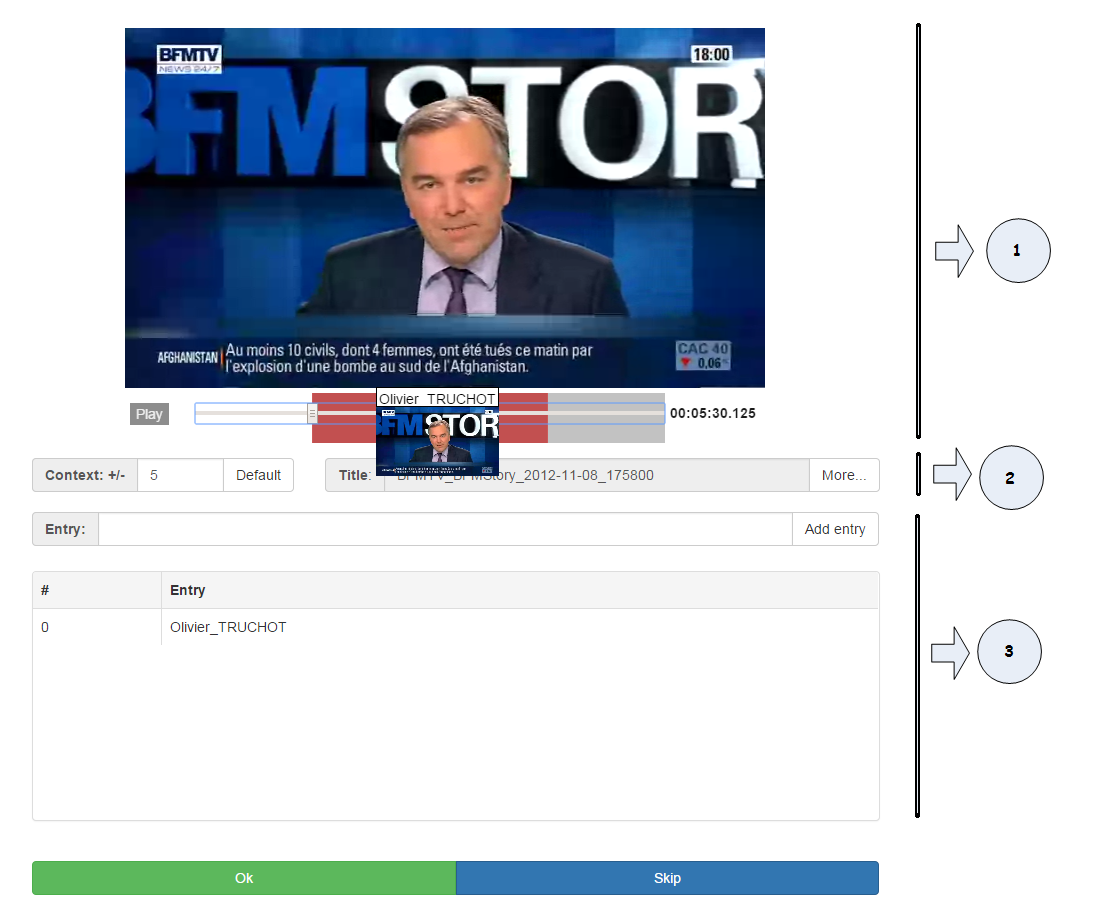
\includegraphics[width=0.5\textwidth]{camomile_ui.png}
	\caption{Overview of the web front-end UI. \emph{1)} Video player displaying the shot/frame to annotate and the synchronized "context bar".\emph{2)} The "context bar" configuration and the video/frame labe and description.\emph{3)} The textfield where user have to type the annotation and the table displaying all available annotation of this shot/frame.}
	\label{fig:front-end-UI}

\end{figure}


An overview of our visual tool is shown in figure~\ref{fig:front-end-UI}. Its components, described later, are implemented with SVG drawing primitives and html elements, that are linked to the data using the D3.js Javascript library \cite{d3js}. The angular.js framework \cite{angularjs} is also used to easily integrate a coordinated SVG context view. The latest version of our tool is available at \cite{url-front-end}.

Though there are two main use cases, explain in Section 2.2.1 and 2.2.2, components are mainly the same for both: the shot or the frame to annotate is displayed in a html5 video player, its title is shown under the player, and when available, a description of it can be shown by clicking a description is available by clicking a button. In order to type the annotation and to point existing data, a textfield and a table are present under the player.\\

Two use cases were defined by the LIG. For each one, a user will run through a list of task (i.e. giving the name and first name of a person). Everytime a task is completed, the UI will load the next one.

\subsubsection{Annotate shot}
In the first use case, a user have to be able to give the identity of a speaking person in a video part, and to navigate through it. He may also want to see some existing annotation upon the shot, as context.\\
In order to display this context, we add wat we called the context bar, a video slider on which we add some layer representing the current annotation to do, and others close to it. A tooltip has also been added on each layer, giving as clue the a thumbnail of the annotation start and the name that may have been given.\\
It is also possible to add seconds in front and after the shot to be able to look for already filled annotation with may be the same person speaking, which may help the user to complete his task.

\subsubsection{Annotate head}
The second one corresponds to give the identity of a on screen appearing person. This time, we thought there was no need to scroll through the video, so only the correspong frame is dislayed to the user. As many person can be on screen, we had to help user to figure out which one have to be identified. That's why we add a layer on the frame, on which we drew a red square surronding the head of the right person.\\

%Resp : LIST

      \subsection{Active learning backend}
(présenter l'approche LIG - retraining and adaptation - et pointer sur le lien github précis - y passer plus de temps 

Resp : Matheusz

      \subsection{Compatibility with other annotation tools}
voir si on ajoute une partie comme ça ou pas?

Resp : LIMSI



  \section{Dry run evaluation}
      \subsection{Use case : multimodal speaker annotation}
     
décrire la tâche et les participants à l'expe

Resp : Mateusz
      
      \subsection{Quantitative analysis}
    
stats présentés par Matheusz au meeting de Madrid

Resp : Mateusz
  
     \subsection{Qualitative analysis}
    
%Analyse des resultats du Survey

During the survey, participants had to fill a form to give some  feedback about the web front-end. This was done using Google forms \cite{url-google-forms}. The form is available on \cite{url-list-form}, and the results are visible at \cite{url-list-form-results}.

If the users were mainly satisfied with the front-end, they pointed out some features that have to be improved. As examples, some tooltips or titles had to be added to improve the clarity of the UI, which have already been done since the survey. They also brought up that some component have to be revamped. The "context bar" is an instance of component on which we have to work. As a short term solution, we chose to add the thumbnail displaying a capture of the person concerned by the annotation, but this component will be totally rethought later.
%resp : LIST




  \section{Conclusion}
  
    \subsection{Supporting data files}

description vidéo démo soumise en même temps que le papier
résumé code github pointé ?    

resp : All

    \subsection{Live demo scenario}

décrire précisément ce qui sera présenté à Dresde en Sept 2015

  
  \newpage
  \eightpt
  \bibliographystyle{IEEEtran}
  
  \bibliography{Camomile}

\end{document}
